\chapter*{Introduction}\addcontentsline{toc}{chapter}{Introduction}
Amidst the countless stars and galaxies we observe in the Universe lie 
undetected structures of dark matter, orders of magnitude larger than 
the luminous objects they engulf. These vast invisible structures began 
in the very early Universe, as quantum fluctuations in the aftermath of 
the Big Bang. During the subsequent period of inflation, these primordial fluctations 
were amplified by the accelerated expansion of the Universe and then 
propagated through gravitational instability for billions of years. 

Despite constituting most of the matter in the Universe, dark matter 
has yet to be directly observed. In fact, it can only be studied through 
its gravitational interactions with luminous baryons, the matter of
stars, galaxies, and celestial objects that emit light. 
In a way, the galaxies we observe in the cosmic volumes probed by our 
telescopes act as illuminated beacons tracing the vast dark matter 
terrains of the Universe.

Over the past decade, spectroscopic redshift surveys like the 
Sloan Digital Sky Survey III Baryon Oscillation Spectroscopic Survey 
(BOSS; \citealt{Anderson:2012aa, Dawson:2013aa}) have 
exploited these galactic beacons to map out cosmic structures
of the Universe. Precise measurements of distance and growth 
of large-scale structure (LSS) from these surveys, provide tests 
of cosmological models that describe the content, geometry and history 
of the Universe. 
The next leap in galaxy surveys will continue to expand the cosmic 
volumes probed by galaxies. These observations have the potential 
to constrain cosmological parameters with unprecedented precision. 
In the following secitons, I briefly introduce how observations from galaxy
redshift surveys can be used to test cosmological models, 
General Relativity, and particle physics beyond the Standard Model.


%In this disseration, I address major methodological challenges in 
%analyzing LSS with galaxies 

%Through these galaxies, we can explore the properties of the underlying dark matter
%and the growth of their structure. Measurements that quantify these properties allow us to make
%precise calculations of cosmological parameters, which quantify the content, geometry, and
%expansion history of the Universe. Ultimately the constraints we measure on these parameters,
%enlighten us on the properties of dark energy, which remains one of the most crucial unsolved
%questions in cosmology. Certainly these precise cosmological measurements require a profound
%understanding of the formation and evolution of galaxies. Unfortunately there is no clear
%narrative of galaxy formation and evolution due to the complex, non-linear, and stochastic nature
%of the physical processes that govern them.

%In fact, galaxy formation and evolution remain another central unsolved questions in
%astrophysics and cosmology. However, since galaxies are enveloped in the massive gravitational
%wells of their host dark matter structures, the underlying dark matter of galaxies undoubtedly
%plays a crucial role in their formation and evolution. Therefore, with its implications on the most
%crucial questions in both cosmology and our understanding of galaxies, the interactions between
%galaxies and their host dark matter environments pose some of the most impactful questions,
%questions that I seek to answer in my dissertation. 


\section{Large Scale Structure in $\Lambda$CDM} \label{sec:lss}
From the early Universe, primordial quantum fluctuations grow into the 
large-scale structures of the Universe we observe today through gravitational 
instability over different epochs of cosmic history. In this section, I briefly 
describe the simplified ({\em linear}) theory of this evolution and explain core 
concepts of LSS cosmology using galaxies. Lets begin by defining the matter 
overdensity field (or density fluctuation) at comoving position $\bm{r}$: 
\beq \label{eq:delta}
\delta(\bm{r}) = \frac{\rho(\bm{r}) - \bar{\rho}}{\bar{\rho}}, 
\eeq
where $\rho(\bm{r})$ is the density field and $\bar{\rho}$ is the mean 
density. Then, in Fourier space the density fluctuation becomes 
\beq
\delta(\bm{k}) = \int \frac{{\rm d^3}\bm{r}}{(2\pi)^3}\; e^{-i\bm{k}\cdot\bm{r}}\;\delta(\bm{r}),
\eeq
the Fourier transform of $\delta(\bm{r})$. 
For describing the evolution of the overdensity field, Fourier space is often 
favored because, as derived later in the section, the Fourier modes of 
$\delta$ evolve independently on large scales -- \emph{i.e.} in linear theory.
The information in the overdensity field is often quantified using its 
$N$-point statistics \citep{peebles80, Bernardeau:2002aa, DodelsonBook}. 
In fact, the two-point statistic is one of the most commonly used tool in 
large scale structure studies. This two-point statistic, which is also 
referred to as the correlation function, is defined as 
\beq
\xi(\bm{r}) = \langle \delta(\bm{x})\delta(\bm{x} +  \bm{r}) \rangle
\eeq
and in Fourier space as
\beq
\langle \delta(\bm{k})\delta(\bm{k'}) \rangle = (2\pi)^3 P(\bm{k})\;\delta^{D}(\bm{k}+\bm{k'}).
\eeq
$\delta^{D}$ is the Dirac delta function and $P(\bm{k})$ is the two-point statistic in 
Fourier space -- the {\em powerspectrum}. $P(\bm{k})$ is the Fourier transform of 
$\xi(\bm{r})$ and, in principle, they contain the same information. 
In practice, however, analyzing $\xi(\bm{r})$ and $P(\bm{k})$ carry different 
caveats~\citep{Feldman:1994aa}. Throughout this dissertation, I will mainly focus 
on the powerspectrum. 

Now in order to determine the evolution of the matter overdensity field
(on sub-horizon scales) consider pressureless dark matter, which consistutes 
most of the matter in the Universe. From the continuity, Euler, and Poisson equations
\beqa 
\frac{\partial \rho}{\partial t} + \nabla \cdot \rho \; \bm{u} = 0  \\ 
\frac{\partial \bm{u} }{\partial t} + (\bm{u} \cdot \nabla) \cdot \bm{u} - \nabla\Phi = 0 \\ 
\nabla^2\Phi - 4 \pi G \rho = 0 
\eeqa
its equation of motion can be derived
\beq \label{eq:meszaros}
\frac{\partial^2 \delta}{\partial t^2} + 2 \frac{\dot{a}}{a} \frac{\partial \delta}{\partial t} - 4 \pi G \bar{\rho}\;\delta = 0.
\eeq
$\bm{u}$ is the velocity field, $\Phi$ is the gravitational potential, and $a$ 
is the scale factor. For a detailed derivation I refer readers to 
\cite{peebles80} and \cite{DodelsonBook}. This equation, a second order differential 
equation. Therefore, the solution can be written as 
\beq 
\delta(\bm{r}, t) = D^{(+)}(t) A(\bm{r}) + D^{(-)}(t) B(\bm{r}).
\eeq
The density flucation has two components: a growing mode $D^{(+)}$ and a decaying 
mode $D^{(-)}$. The decaying mode, as its name suggests, decreases with time 
and its contribution becomes negligible in the late Universe leaving only the 
growing mode. To quantify the evolution of the growing mode $D^{(+)}$, one 
commonly used quantity is the ``growth rate of structure'': 
\beq \label{eq:f_growth}
f = \frac{ d\; {\rm ln}\;D^{(+)}}{d\; {\rm ln}\;a}. 
\eeq
This growth rate of structure is a key quantity in LSS cosmology for testing different 
cosmological models and theories of gravity. $f$ will be discussed further in 
Section~\ref{sec:rsd}.

In addition to the their gravitation evolution, the density fluctuations 
evolve through different epochs in cosmic history: inflation, 
radiation-dominated era, matter-radiation equality, and matter-dominated era. Each of 
these periods leave an imprint on the evolution of $\delta$. In Fig.~\ref{fig:lifo}, 
I mark the eras in the early Universe and plot how the physical scale of 
the Universe, represented by the Hubble radius, evolves with the scale factor $a$. 

During inflation, the Hubble radius remains constant. Afterwards the Universe 
becomes radiation dominated. Based on the Friedmann equations the Hubble radius 
during the radiation dominated era is approximately $\propto a^{2}$. After a period 
when radiation and matter have comparable energy densities, the Universe 
becomes matter dominated where the Hubble radius is approximately $\propto a^{3/2}$. 
Meanwhile, the physical scale of perturbations is $\lambda_{phys} = \lambda_{comov}\ a(t)$ 
and thus $\propto a(t)$. As Fig.~\ref{fig:lifo} schematically illustrates, 
perturbations exit the Hubble radius during inflation then 
reenter the Hubble radius later on. 
Depending on the physical scale of the perturbation, it enters either
during the radiation-dominated era (smaller scale) or matter-dominated era (larger scale). 

The physical scale of perturbations that enter the horizon at the time of 
matter-radiation equality, where $a(t) = a_{eq}$, is $\lambda_{eq} \sim 500\;h^{-1}{\rm Mpc}$.
Then perturbations that enter before the matter-radiation equality 
have physical scales $\lambda_{phys} < \lambda_{eq}$ and since they enter
during the radiation dominated era, these smaller scale perturbations 
are effectively frozen and hence their growth is suppressed.
On the other hand, the larger scale perturbations with $\lambda_{phys} > \lambda_{eq}$
enter after matter-radiation equality during the matter dominated epoch. These 
perturbations do {\em not} experience the suppression of growth of the radiation 
dominated era. The net effect on the overdensity as it goes through these epochs 
is the suppression of growth on scales smaller than $\lambda_{eq}$, or $k_{eq}$ in 
Fourier space, by a factor of $\sim k^4$. In practice, this scale dependent 
evolution of the density fluctuation is quantified through the 
``transfer function'' $T(k)$~\citep{Eisenstein:1998aa, Eisenstein:1999aa}. 

\begin{figure*}
\begin{center}
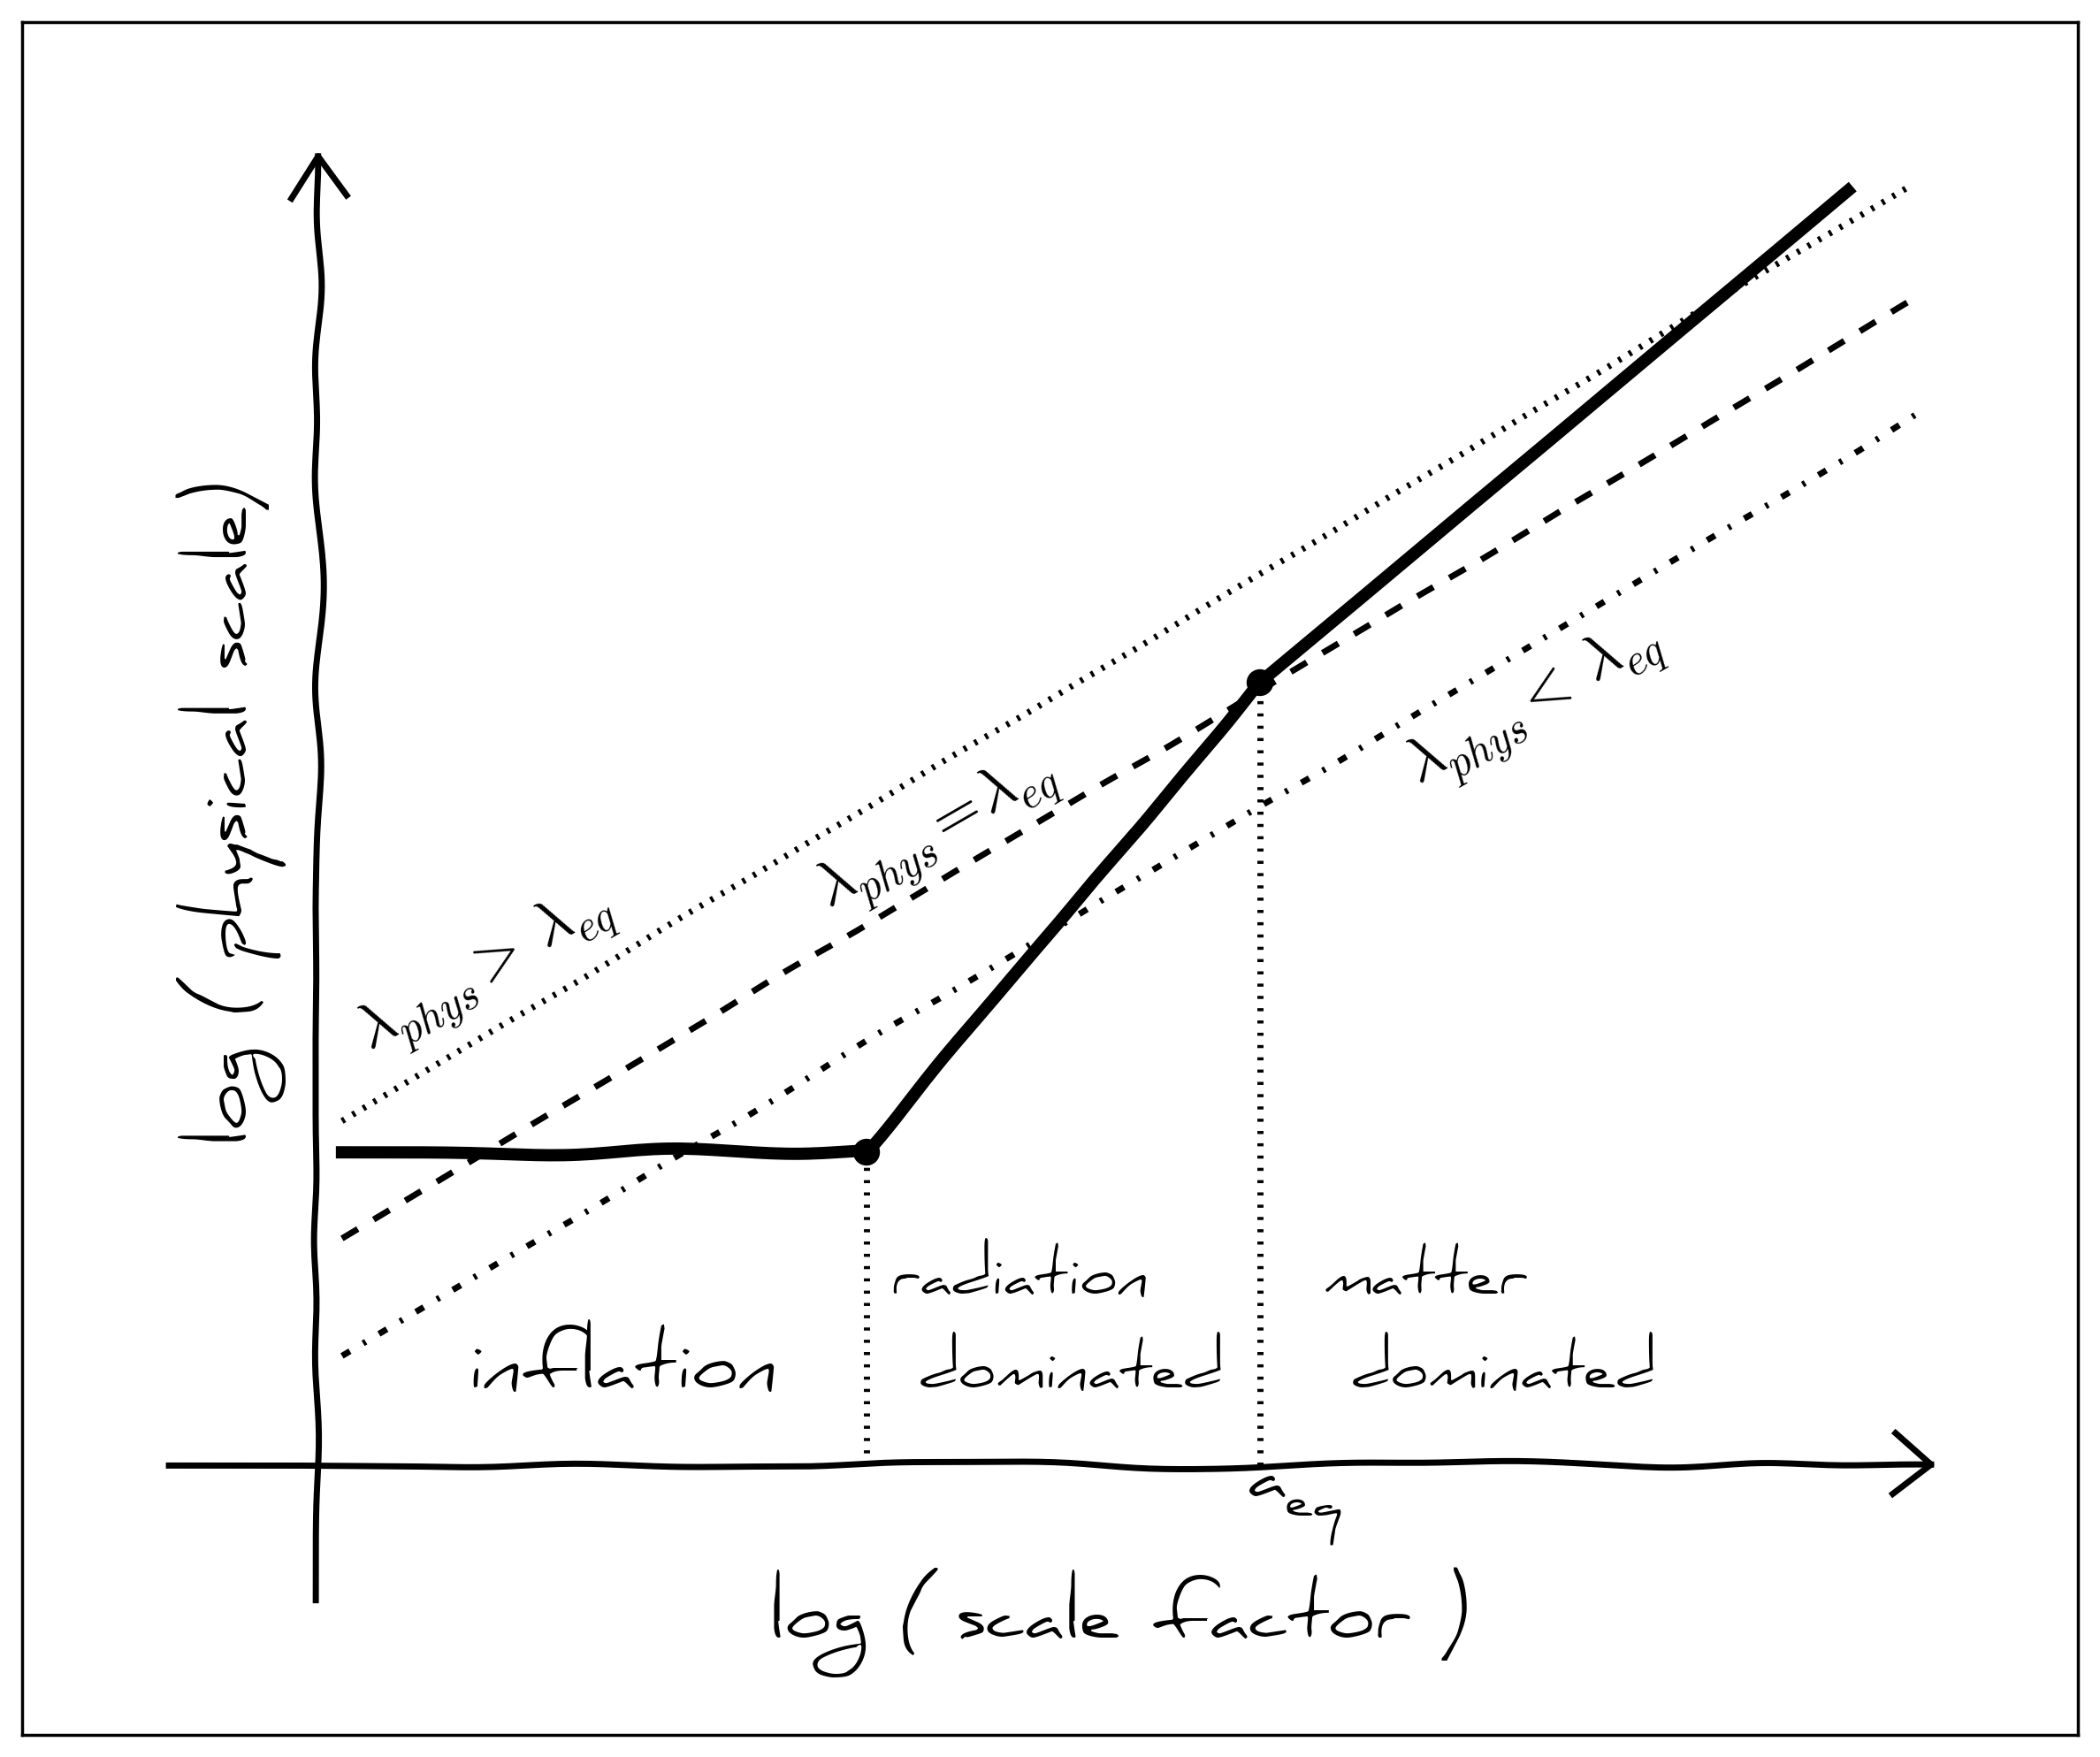
\includegraphics[width=\textwidth]{figs/lifo.png}
\caption{Schematic diagram that illustrates the evolution of the density 
fluctuations in the early Universe through inflation, radiation-dominated epoch, 
matter-radiation equality, and matter-dominated epoch. The evolution of the 
Hubble radius (solid line) remains flat during inflation (flat), scales by 
$\propto a^2$ during radiation domination, and $\propto a^{3/2}$ during matter
domination. $a_{eq}$ marks matter radiation equality. The physical lengths of
three constant comoving scales are marked by dashed, dotted, and dot-dashed
lines. The dashed line represents physical lengths of perturbations 
that enter the horizon during matter-radiation equality $\lambda_{phys}=\lambda_{eq}$. 
The dot-dashed line mark perturbations that enter the horizon during radiation 
domination with $\lambda_{phys} < \lambda_{eq}$.  The dotted line mark 
perturbations that enter the horizon during matter domination with 
$\lambda_{phys} > \lambda_{eq}$. As described in the text, the growth of perturbations 
with $\lambda_{phys} < \lambda_{eq}$ are suppressed because they enter the 
horizon during the radiation dominated era. The evolution of the density 
perturbation through these epochs are quantified through the transfer function $T(k)$.} 
\label{fig:lifo}
\end{center}
\end{figure*}

The density fluctuations after inflation can be summarized by the powerspectrum: 
\beq
P_{\rm inf}(k) \propto k^{n_s}
\eeq
where $n_s$, the spectral tilt of the primordial powerspectrum, is measured to be 
$\sim 1$ \citep{Harrison:1970aa, Peebles:1970, Zeldovich:1972, Komatsu:2011aa}.
Then, the powerspectrum of the density fluctuation in the late Universe can be 
expressed as 
\beq
P(k) \propto k^{n_s} \; T^2(k) \; D^2(k).
\eeq
where $D(k) \equiv D^{(+)}$ is the growth function from earlier this section. 
Through the cosmological models and parameters, which predict 
$T(k)$ and $D(k)$, we predict the powerspectrum of the density fluctuation. Then 
these predictions can then be compared to measurements made from observations in 
order to produce constraints on cosmological parameters, better understand dark 
energy, and test theories of gravity. 

Unfortunately, most of the matter in the Universe is in the form of dark 
matter and does not interact with radiation, so observers cannot measure the 
spatial/clustering statistics of dark matter directly. 
Instead, we measure the clustering of galaxies or quasars, which trace
the underlying matter distribution. The smoothed galaxy/quasar density field 
can be  approximated by a local function of the matter density field
\beq
\delta_g(\bm{r}) = f( \delta(\bm{r})). 
\eeq
$f(\delta(\bm{r}))$ can then be expanded Taylor series~\citep{Fry:1993}:
\beq
\delta_g({\bf r}) = \sum\limits_{k=0}^{\infty} \frac{b_k}{k!} \delta^k 
\eeq
where $b_0$ is chosen so that $\langle \delta_g \rangle = 0$ and $b_1$ is referred to as 
the linear bias factor. To linear order, 
\beq
P_g(k) = b_1^2 P(k). 
\eeq
The primary galaxy subpopulation used in LSS studies so far are luminous 
red galaxies~\citep{Eisenstein:2001aa, Dawson:2013aa}. These galaxies have $b_1 > 1$,
which makes them {\em biased} tracers of the matter 
distribution~\citep{Zehavi:2005aa, Sheldon:2009aa,Gaztanaga:2009aa, Zhai:2016aa}.
Luminous galaxies reside in larger potential wells. The peaks of the density fluctuation
have stronger clustering properties than the overall overdensity field~\citep{Manera:2010aa}.

Based on the derivation of this section, once we have the spatial 
distribution of galaxies or quasars, we can derive the clustering of the matter
distribution and then infer cosmological constraints. In practice, however, a
number of factors complicate this procedure. One major complication is redshift-space
distortions, which will be discussed in the next section.

\section{Redshift-Space Distortions} \label{sec:rsd}
Spectroscopic redshifts surveys, such as 2dF Galaxy Redshift Survey~\citep{Colless:1999aa}, 
Sloan Digital Sky Survey, and BOSS, have mapped out millions of distant galaxies. 
Current surveys such as Extended Baryon Oscillation 
Spectroscopic Survey (eBOSS; \citealt{Dawson:2015aa}), and future surveys such as 
the Dark Energy Survey Instrument (DESI; \citealt{Schlegel:2011aa, Morales:2012aa, Makarem:2014aa}) 
and the Subaru Prime Focus Spectrograph (PFS; \citealt{Takada:2014aa}), will 
continue to map out millions more. These surveys dominate LSS studies and have/will 
been critical for inferring precise cosmological constraints. As their name suggest, 
however, these {\em redshift} surveys do not directly measure the acutal position of 
galaxies. Instead they measure the angular positions (right ascension and declination) 
and redshifts of galaxies. 

These redshifts are a combined measurement of the recession velocities due to 
the expansion of the Universe and the peculiar velocities of the galaxies:
\beq
z_{obv} = z_{true} +  \frac{v_{pec}}{c}.
\eeq 
The galaxy comoving positions derived from the angular positions and redshifts are then
in {\em redshift-space} and ``distorted'' compared to real-space comoving positions by 
\beq
\bm{s} = \bm{x} +  \frac{\bm{v}_{pec} \cdot \hat{n}}{H_0}
\eeq 
where $\hat{n}$ is the unit vector along the line-of-sight. Thankfully, all hope is not 
lost. 

The peculiar velocities of galaxies are directly related to the total 
matter distribution, since galaxies can be thought of as test particles in a 
gravitational field. Using this relation, \cite{Kaiser:1984aa} derived an 
approximation for the distortion caused by the coherent infall of galaxies 
onto overdense regions in redshift space. This redshift-space 
distortion (RSD), often referred to as the Kaiser effect, causes observations of 
overdense regions
to appear squashed along the line of sight in redshift-space. Galaxies around an
overdense region that are closest to the observer on Earth are moving towards the center of the 
overdense region and away from the observer. So in they appear farther away than 
their true position. Galaxies on the other side are moving towards both the overdense 
region and the observer, so they appear closer to us in redshift-space. 

The relation between the overdensity field in redshift-space can be 
derived from the continuity equation and the distant observer approximation, 
\beq
\delta^{(s)}(\bm{k}) = (1 + f \mu^2) \delta(\bm{k}).
\eeq
$f$ is the growth rate of structure (Eq.~\ref{eq:f_growth}) and 
$\mu = \bm{k} \cdot \hat{n} / k$, cosine of the angle between $\bm{k}$ and 
the line-of-sight. In corporating the Kaiser effect into the galaxy bias model 
from Section~\ref{sec:lss}, the galaxy/quasar overdensity field in 
redshift-space becomes
\beq
\delta_g^{(s)}(\bm{k}) = (b_1 + f \mu^2) \delta(\bm{k}).
\eeq
The redshift-space powerspectrum of the galaxy overdensity field can then be
written as 
\beq
P_g^{(s)}(k, \mu) = (b_1 + f \mu^2)^2 P(\bm{k}).
\eeq
On large scales and with small overdensities, the effect of redshift-space 
distoritons is well described by the Kaiser effect. On small scales with large
overdensities things get a little more complicated. 

The random peculiar velocities of galaxies in gravitationally bound structures 
such as clusters cause their position in redshift-space to be smeared out to 
larger scales along the line-of-sight. This effect can easily be identified by 
eye in galaxy redshift maps where the elongations of the galaxy positions along the 
line-of-sight resemble fingers pointing towards the observer. Aptly this 
redshift-space distortion is referred to as the ``fingers-of-god''. Its impact on the 
powerspectrum, is empirically modeled and typical quantified using an overall exponential 
factor \citep[][]{Jackson:1972aa,Scoccimarro:2004aa,Taruya:2010aa,Beutler:2016aa}. 
Including both RSDs from the Kaiser effect and the fingers-of-god, the 
redshift-space powerspectrum is then 
\beq \label{eq:pk_rsd}
P_g^{(s)}(k, \mu) \approx e^{-f^2 \sigma_v^2 \mu^2 k^2} (b_1 + f \mu^2)^2 P(k)
\eeq
where $\sigma_v$ is a paramter quantifying the strength of the effect and is usually
left as a free parameter in analyses. 

Eq.~\ref{eq:pk_rsd} reveals the $f$ dependence in RSDs. RSD analyses in 
LSS studies exploit this dependence by measuring the impact of RSDs on 
the powerspectrum to constrain $f$. 
Consider the Legendre expansion of $P_g^{(s)}(k, \mu)$, 
\beq
P_g^{(s)}(k, \mu) = \sum\limits_{\ell=0, 2, 4 ...} \mathcal{L}_\ell(\mu) P_g^\ell(k). 
\eeq
Each of powerspectrum ``multipole'' of this expansion is then  
\beq
P_g^{\ell}(k) = \frac{2 \ell + 1}{2} \int\limits_{-1}^{1} {\rm d}\mu \; P_g^{(s)}(k, \mu)\; \mathcal{L}_\ell(\mu).
\eeq
The RSD factor in the  powerspectrum multipoles for $\ell= 0$ (monopole) and $2$ (quadrupole)
are 
\beqa
P_g^0 (k) &=& (b_1^2 + \frac{2}{3} f b_1 + \frac{1}{5}f^2) P(k) \\
P_g^2 (k) &=& (\frac{4}{3} f b_1 + \frac{4}{7} f^2) P(k). 
\eeqa
For simplicity, we neglect the fingers-of-god, which does not significantly impact larger scales. 
Taking the ratio of the quadrupole over the monopole, 
\beq \label{eq:multipole_ratio}
\frac{P_g^2}{P_g^0} = \frac{\frac{4}{3} f b_1 + \frac{4}{7} f^2}{b_1^2 + \frac{2}{3} f b_1 + \frac{1}{5}f^2},
\eeq
we can in principle eliminate the dependence on scale and extract information on $f$. 
Of course in practice the simplified derivations of this section break down. Instead
of the simple linear theory theoretical models I derived, models of $P_g^{(s)}$ 
are derived using perturbation theory and incorporate more sophisticated RSD and bias 
models~\citep[][]{Bernardeau:2002aa, Scoccimarro:2004aa, Taruya:2010aa, Nishimichi:2011aa, Taruya:2013aa, Taruya:2014aa, Beutler:2016aa}. 
These models are then compared to the observed $P_g$ multipoles from galaxy surveys 
in order to derive constraints on cosmological parmaeters such as $f$. 
%illustrates how the distortions caused by RSDs allow us to extract information of $f$ through measurements of the redshift-space galaxy powerspectrum!  

\section{Weighting Neutrinos with Galaxies} \label{sec:mneut}
Beyond inferring the growth rate of structure, which 
can be used to test GR and modified gravity scenarios, galaxy clustering
also provides a unique window to probe fundamental physics beyond the 
standard model. 
In the derivations of Sections~\ref{sec:lss} and~\ref{sec:rsd} we focused 
on how the dark matter density fluctuations of evolves. This is an excellent
approximation because dark matter consistutes the majority of matter in the 
Universe. However, it negelects some of the more detailed imprints on 
LSS from other components of matter -- \emph{i.e.} neutrinos, which  
oscillation and detection experiments have \emph{very} convincingly 
(Nobel Prize in Physics 2015) confirmed is {\em not} massless~\citep[][]{
Hu:1998aa, Lesgourgues:2012aa, Lesgourgues:2013aa, Lesgourgues:2014aa}.
%(\todo{Beringer et al. 2012,Lesgourges, 2012, 2013})

In the very early Universe, neutrinos are relativistic and coupled to the 
primordial plamsa. Later they decouple from the plasma, while they are still 
ultra-relativistic and redshift. At this point, they do not 
contribute to the energy density of matter but instead radiation. Eventually during 
matter domination era, neutrinos become non-relativistic and then contribute 
to the matter energy density acting as ``warm/hot'' dark matter.
After decoupling from the primoridal plasma, neutrinos are effectively a
collisionless fluid, where the individual particles free-stream with 
characteristic velocities defined by their thermal velocity. Earlier on 
when they are relativistic, their free-streaming scale is simply 
equal to the Hubble radius. Later when they are non-relativistic, 
their characteristic velocity is approximately  
\beq
v_{\rm th} \approx 158 (1 + z) \left(\frac{1 {\rm eV}}{m} \right) \; \; {\rm km \; s^{-1}}
\eeq
and the free-streaming scale can be derived in an analogous way as the 
Jean's length derivation: 
\beq
\lambda_{\rm FS} = 2 \pi \sqrt{\frac{2}{3}} \left( \frac{v_{\rm th}}{H} \right)
\eeq
or 
\beq \label{eq:kfs}
k_{\rm FS} = \frac{2\pi a}{\lambda_{\rm FS}} \approx  0.82 \frac{\sqrt{\Omega_\Lambda + \Omega_m(1+z)^3}}{(1+z)^2} \left(\frac{m_\nu}{1\;{\rm eV}} \right).
\eeq
where $\Omega_\Lambda$ and $\Omega_m$ are the current cosmological constant and matter 
density fractions, respectively.

Neutrinos leave two main imprints on LSS. In the early Universe they contribute
to the radiation energy density but later, they contribute to the matter energy 
density. As described in 
Section~\ref{sec:lss}, matter-radiation equality marks the turning point in 
suppression of growth of structure, quantified by $T(k)$. The transition of 
neutrinos from radiation to matter impacts $a_{eq}$ and thus impacts $T(k)$ by 
shifting the turning point of the cold dark matter (CDM) only powerspectrum. 
Even after becoming non-relativistic, neutrinos still do not contribute to the
clustering of matter on scale smaller than $k_{\rm FS}$. The impact of this scale dependent 
suppression of clustering, can be analytically estimated for the matter powerspectrum 
\citep{Bird:2012aa}: 
\beq
\frac{\Delta P}{P} = \frac{P^{f_\nu \neq 0} - P^{f_\nu = 0}}{P^{f_\nu = 0}} \approx - 8 f_\nu \;\;\;\; {\rm for}\;\; k \gg k_{\rm FS}.
\eeq
where $f_\nu$ is the ratio of the neutrino energy density over that of matter 
($\Omega_\nu / \Omega_m$).

The total mass of neutrinos (\mneut) dictates the strength of these imprints and  
can therefore be constrained by the shape of the powerspectrum. The same tools 
used for analyzing RSDs and measuring the growth rate of structure can also be 
used to measure \mneut\; from observations of galaxy 
surveys~\citep{Hu:1998ab, Costanzi:2013aa, Villaescusa:2015aa, Cuesta:2016ab}.
Based on forecasts, the next galaxy surveys such as 
DESI\footnote{DESI \textit{Final Design Report} (FDR): \url{http://desi.lbl.gov/tdr/}} 
have the potential to infer the most stringent constraints on 
\mneut -- $\sigma_{\sum m_\nu} \sim 0.03\;{\rm eV}$. Such constraints would 
trump the sensitivity of particle physics experiments~\citep[][]{Wolf_Katrin}
and have the potential to distinguish
between the normal or invereted neutrino mass hierarchy and reveal physics
beyond the Standard Model.

\section{Analyzing Galaxy Clustering}
%Beyond the general description and derivation of the redshift-space galaxy powerspectrum, the rest of galaxy clustering analysis in LSS studies follows the standard approach to Bayesian parameter inference. 
In the previous sections, I laid out the theoretical framework for LSS analysis 
using galaxy clustering. As I alluded earlier, the models and predictions of 
this theoretical framework can be compared to observations to derive constraints
on parameters of interest. In this section I describe the statistical framework 
for comparing the theoretical models to observations from galaxy surveys. 
The ultimate goal of galaxy clustering analyses is to derive 
probability distributions of the cosmological parameters (\emph{e.g.} $f$, \mneut)
given the data from observations. 
The standard approach to deriving this {\em posterior} probability distribution is using 
Bayesian parameter inference. Based on Bayes theorem, the posterior probability distribution 
can be expressed as 
\beq
P(\bm{\theta}| \bm{D}) = \frac{P(\bm{D}|\bm{\theta}) P(\bm{\theta})}{P(\bm{D})}.
\eeq
$\bm{D}$ and $\bm{\theta}$ refer to observations and cosmological parameters, respectively. 
$P(\bm{D}|\bm{\theta})$, the probability distribution function for the observation $\bm{D}$ 
given model parameters $\bm{\theta}$, is the {\em likelihood function} ($\mathcal{L}$). 
$P(\bm{\theta})$ is the {\em prior} probability distribution function. Lastly, 
$P(\bm{D})$ is the ``evidence'', which for our purposes is just a normalization 
factor independent of $\bm{\theta}$. The equation is more commonly simplified as 
\beqa \label{eq:bayes} 
P(\bm{\theta}|\bm{D}) &\propto& P(\bm{D}|\bm{\theta}) \; P(\bm{\theta}) \\
{\rm posterior} &\propto& {\rm likelihood}\; \times \; {\rm prior}.
\eeqa

In the context of galaxy clustering analyses and LSS cosmology in general, the likelihood 
function is {\em typically} assumed to have Gaussian function form and calculated as 
\beq \label{eq:likelihood}
P(\bm{D}|\bm{\theta}) = \mathcal{L} = \frac{1}{(2\pi)^{N_d/2}\; {\rm det}\bm{C}^{1/2}}\; {\rm exp}\left[ -\frac{1}{2} (\bm{D} - F(\bm{\theta}))^T \bm{C}^{-1} (\bm{D} - F(\bm{\theta}))\right].
\eeq
$\bm{D}$ is data observed and measured from galaxy surveys with dimension $N_d$. 
$F(\bm{\theta})$ is the model prediction of the observable (\emph{e.g.} 
$P_g^{(s)}$) generated from cosmological parameters $\bm{\theta}$, described in 
earlier sections. And $\bm{C}$ is the covariance matrix. 

A number of different methods are used to estimate the covariance matrix. For instance, 
efforts to analytically estimate the covariance matrix from theory have been made in 
the past~\citep{Hamilton:2006aa, Pope:2008aa, dePutter:2012aa}. However, 
non-linear evolution, shot-noise, RSDs, and mapping between galaxies and matter
complicate accurate estimations. Jack-knife resampling~\citep{Shao:1995aa}, 
a commonly used method in astronomy for estimating covariances directly from data 
have also been used. However, the method requires a number of arbitrary choices 
and cannot account for fluctuations on the scale of the survey~\citep{Norberg:2009aa}.
Instead, the latest analyses estimate $\bm{C}$ from galaxy mock catalogs generated 
from $N$-body simulations. For accurate estimation, an order of $\sim 1000$ mock
galaxy catalogs are required in the analysis~\citep{Scoccimarro:2002aa, McBridge:2011aa, 
Anderson:2012aa, Manera:2013aa, Rodriguez-Torres:2015aa, Kitaura:2016aa, Beutler:2016aa}
Developing fast and accurate galaxy mock catalogs for LSS analyses has now become a 
subfield of its own. As an added detail, in standard analyses, in order to 
account for biases in the $\bm{C}$ estimates, include a correction -- the Hartlap factor -- 
to the covariance matrix estimate~\citep{hartlap2007}.

From $\bm{D}$, $F(\bm{\theta})$, and $\bm{C}$ we can evalulate an estimate of the 
likelihood function. From the likelihood,
since the prior probability distribution is chosen {\em a priori}, the posterior 
probability distribution functions of the cosmological parameters is essentially already 
evaluated. In practice, the posterior distribution is not evaluated at all points in 
parameter space, but rather sampled using a sampler such as a Markov Chain Monte 
Carlo sampler \citep[\emph{e.g.} $\mathtt{emcee}$][]{emcee}.

From the galaxy clustering analysis described in this chapter, the latest 
galaxy surveys have produced some remarkable constraints on cosmological parameters. 
From the SDSS and BOSS surveys, measurements of the powerspectrum multipoles 
along with analogous configure-space analyses have yielded a number of constraints 
on $f\sigma_8$~\citep{Reid:2012aa, Oka:2014aa, Beutler:2014aa, Alam:2015aa, Alam:2016aa, Beutler:2016aa}, 
where $\sigma_8$ 
is the amplitude of the powerspectrum on the scale of $8\;h^{-1}{\rm Mpc}$. 
Similar to multipoles, powerspectrum wedges have also been used, in both 
Fourier and configuration-spaces, to infer $f\sigma_8$ 
constraints~\citep{Sanchez:2013aa, Sanchez:2016aa, Grieb:2016aa}. 
These $f \sigma_8$ constraints can then be compared to cosmological predictions 
from Cosmic Microwave Background (CMB) experiments such as the Wilkinson
Microwave Anisotropy Probe~\citep{WMAP:2013} and {\em Planck}~\citep{Planck:2014aa}
to test $\Lambda$CDM cosmology and General Relativity. 
The constraints from BOSS are generally consistent $\Lambda$CDM and GR over 
$0.2 < z < 0.75$.  For instance, \cite{Beutler:2016aa} derives 
$f\sigma_8 = 0.482 \pm 0.053, 0.455 \pm 0.050$, and $0.410 \pm 0.042$ from BOSS 
for effective redshift $z_{\rm eff} = 0.38, 0.51$, and $0.61$.
$f \sigma_8$ constraints from galaxy powerpsectrum analyses have also been 
combined with CMB data to constrain \mneut~\citep{Zhao:2013aa, Beutler:2014ab, Gil-Marin:2015aa}.
\cite{Beutler:2014ab}, from combining constraints from galaxy powerspectrum 
analyses with {\em Planck} CMB results, derives the upper bound \mneut$ < 0.51\;{\rm eV}$.

%Cosmological measurements such as galaxy clustering statistics are no longer dominated by uncertainties from statistical precision, but from systematic effects of the measurements. This is a result of the millions of redshifts to distant galaxies that have been obtained through redshift surveys such as the 2dF Galaxy Redshift Survey (2dFGRS; \citealt{Colless:1999aa}) and the Sloan Digital Sky Survey III Baryon Oscillation Spectroscopic Survey 
Ongoing and future surveys, such as eBOSS, PFS, and DESI, will 
continue to collect many more million redshifts and expand the probed cosmic 
volume by an order of magnitude. These observations have the potential to 
produce cosmological parameter constraints with unprecedented statistical 
precision. The main challenges for realizing their full potential are {\em methodological}.

So far I have focused on LSS analyses using only the galaxy powerspectrum 
-- the two-point statistic of the density fluctuations. Analyses restricted
to just the two-point statistic, however, face a number of limitations. 
The constraints on the growth rate of structure, listed above, have all 
constrained $f \sigma_8$ rather than $f$ alone. The degeneracy 
between $f$ and $\sigma_8$ cannot be broken with $P(k)$ alone. Furthermore, 
the $P(k)$ multipoles in Eq.~\ref{eq:multipole_ratio} illustrate that 
$P(k)$ analyses also suffer from the degeneracy between $f$ and bias 
parameters. 

\begin{figure*}
\begin{center}
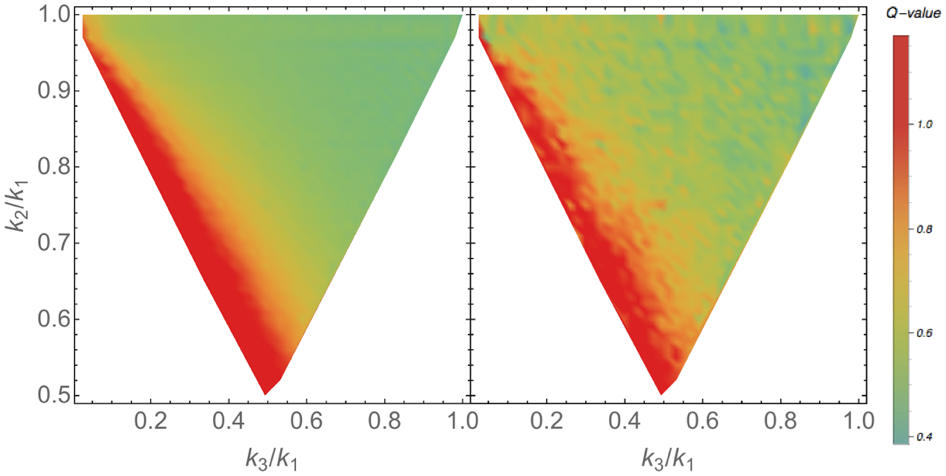
\includegraphics[width=\textwidth]{figs/bisp.png}
\caption{Amplitude of the reduced galaxy bispectrum $Q(k_1, k_2, k_3)$ plotted as a function of 
ratios $k_2/k_1$ and $k_3/k_1$, which describe the triangle configurations. The 
$Q(k_1, k_2, k_3)$ in the left panel is calculated from a perturbation theory model while the 
right panel presents $Q(k_1, k_2, k_3)$ of BOSS Data Release 12 CMASS galaxy sample
using the \cite{Scoccimarro:2015aa} estimator.
}
\label{fig:bisp}
\end{center}
\end{figure*}

The {\em bispectrum} $B(k_1, k_2, k_3)$, the three-point statistic of density
fluctuations, can be used to break the degeneracies among $f$, 
$\sigma_8$, and bias parameters~\citep[][see \citealt{Bernardeau:2002aa} for a review]{Scoccimarro:1998aa, Verde:1998aa, Scoccimarro:2000aa}.
The dependence on triangle configuration in $B(⃗k_1, k_2, k_3)$ 
disentangles contributions from gravitational instability versus 
non-linear biasing of galaxies. Without going into any further detail, 
in Figure\ref{fig:bisp} I present the reduced galaxy bispectrum 
$Q(k_1, k_2, k_3) = B(k_1, k_2, k_3)/(P(k_1)P(k_2) + P(k_2)P(k_3) + P(k_1)P(k_3))$ 
measurement for the BOSS Data Release 12 CMASS (not an acronym) galaxy sample 
(right) and a perturbation theory model (left). The BOSS $Q(k_1, k_2, k_3)$ is 
measured using the \cite{Scoccimarro:2015aa} estimator. 
$P(k)$ and $B(k_1, k_2, k_3)$ measurements from galaxy surveys can be jointly analyzed in order to
derive constraints explicitly on $f$. 

All LSS analyses suffer from observational systematic effects. 
For fiber-fed multi-object spectroscopic surveys 
(\emph{e.g.} SDSS, BOSS, eBOSS, DESI, and PFS) these effects include 
incompleteness from stellar density, incompleteness from seeing, 
fiber collisions, and redshift failures~\citep{Ross:2012aa, Anderson:2012aa}. 
If unaccounted, fiber collisions, for instance, prevent surveys from 
collecting a significant fraction redshifts due to physical constraints 
on the focal plane. As I detail in \chap{fc}, their impact on $P(k)$ 
goes well beyond their angular scale and restricts analysis on small 
scales, which have higher signal-to-noise. 
In addition to diminishing the statistical power of galaxy redshift surveys, 
fiber collisions can also bias constraints on cosmological parameters. 
Fortunately, challenges from observational systematics are often {\em solvable}
\citep[][and \chap{fc}]{Ross:2012aa, Guo:2012aa}.

In Eq.~\ref{eq:likelihood}, the likelihood function assumes a Gaussian functional form
-- a standard assumption in LSS analyses. However, in detail, this assumption cannot 
be correct due to nonlinear gravitational evolution and biasing~\citep{Mo:1996aa, Sommerville:2001aa, Casas-Miranda:2002aa, Bernardeau:2002aa}.
The likelihood also relies on the estimated covariance matrix to capture 
the sample variance of the data. Besides the labor and computational costs 
of required,  simulated mock catalogs used for covariance matrix estimation 
are inaccurate on small scales~(see \citealt{cosmiccode,nifty} and references therein). 
Furthermore, using covariance 
matrix estimates rather than the ``true'' covariance matrix \citep{Sellentin:2016a}
along with systematics impact the likelihood in ways difficult to model. 
Fortunately, evaluating the explicit likelihood is {\em not} necessary for inferring
cosmological parameters. Likelihood-free inferences such as Approximate 
Bayesian Computation (ABC) relax these restrictions and make inference 
possible without making any assumptions on the likelihood.  In \chap{abc}
I combine ABC with a Population Monte Carlo sampler and apply it in the
context of LSS.

As described earlier, galaxies are biased tracers of the 
underlying matter distribution. For more than a decade, halo occupation 
modeling has been the main, and effective, framework for connecting galaxies
to the dark matter structures underneath in galaxy formation and cosmology
studies~\citep{Yang:2003aa, Tinker:2005aa, vandenBosch:2007aa, Zheng:2007aa, 
Conroy:2009aa, Guo:2011aa, Leauthaud:2012aa, Tinker:2013aa, Zu:2015aa}.
The standard halo occupation model
assumes that galaxies reside in dark mater halos and their occupation 
is a function of only the mass of the halo. However, the clustering of dark 
matter halos depend on properties beyond their masses, such as their 
assembly history. If this effect, coined 
{\em halo assembly bias}, propagates to galaxies, it will induce 
{\em galaxy assembly bias} on standard halo occupaiton model and 
significantly impact galaxy clustering 
analyses~\citep[][]{hearin15, Zentner:2016aa, Vakili:2016aa}. 
Therefore, better understanding of the galaxy-halo connection is 
essential for LSS analyses. 

Beyond their utility as tracers for cosmology, galaxies also pose fundamental 
questions regarding how the early homogenous Universe became the heterogenous 
one today. Observations have now firmly established a global view of galaxy 
properties out to $z\sim1$ \citep[\emph{e.g.}][\chap{galenv}]{Blanton:2009aa, Moustakas:2013aa}.
Galaxies roughly fall into two categories: star-forming galaxies and 
quiescent ones with little star formation. The star-forming population 
undergoes significant decline in star formation rate (SFR) over cosmic 
time and significant fractions of them also rapidly ``quench'' their 
star formation and become quiescent. The underlying drivers of this 
evolution, however, are not directly revealed by observations.
Cosmology, which precisely predicts the dark matter evolution, provides 
a framework for answering {\em specific} and {\em tractable} questions 
in galaxy evolution.  In $\Lambda$CDM, structures form 
``hierarchically'' --- smaller ones form earlier and subsequently 
merge to form larger ones. The galaxy population can be positioned in 
this framework with halo occupation in order to constrain key elements 
of their evolution and better understand the galaxy-halo connection 
\citep[][]{Wetzel:2013aa, Wetzel:2014aa, Tinker:2016ab, Tinker:2017aa}. 
In \chap{galhalo}, I use this approach to measure the timescale of star-formation quenching 
in central galaxies. 

In this dissertation, I tackle key methodological challenges in LSS analyses
with galaxy clustering by developing methods to robustly treat systematics (\chap{fc}), 
introducing innovative approaches to inference in LSS studies (\chap{abc}), and 
improving our understanding of the galaxy-halo connection 
(\chapname s~\chapalt{galenv} and~\chapalt{galhalo}). Each Chapter contributes to unlocking 
the full potential of current and future galaxy redshift surveys and will be
critical for testing cosmological models and General Relativity and 
constraining the total neutrino mass. 

\chapname s~\chapalt{fc} and~\chapalt{galenv} have both been refereed and
published in the astronomical literature.
\chapname s~\chapalt{abc} and~\chapalt{galhalo} have both been refereed and accepted 
to the \emph{Monthly Notices of the Royal Astronomical Society} and \emph{The Astrophysical Journal},
respectively. All of these \chapname s were co-authored with collaborators but the majority
of the work and writing in each \chapname\ is mine. Below, I describe my contributions to each \chapname:
\begin{enumerate}

{\item 
For \chap{fc}, I developed the idea for the project in collaboration with Roman
Scoccimarro and Michael Blanton. I implemented the project with contributions 
from Roman Scoccimarro. The project utilized simulation data from Jeremy Tinker
and Sergio Rodr\'{i}guez-Torres. I wrote the paper with additions from 
Roman Scoccimarro and edits by Michael Blanton. 
}

{\item 
For \chap{abc}, I developed the idea for the project in collaboration with 
Mohammadjavad Vakili, Andrew Hearin, and David Hogg. I implemented the project 
with Mohammadjavad Vakili and contributions from Andrew Hearin and Kilian Walsh.
The project utilized software written by Andrew Hearin and Duncan Campell. 
I wrote the paper together with Mohammadjavad Vakili with additions from
Andrew Hearin, David Hogg, and Kilian Walsh.
}

{\item 
For \chap{galenv}, I developed the idea for the project in collaboration with 
Michael Blanton. I implemented the project using catalogs constructed by 
John Moustakas from observations made by the PRIMUS collaboration (Alison Coil,
Richard Cool, Daniel Eisenstein, Ramin Skibb, Kenneth Wong, and Guangtun Zhu).
I wrote the paper with additions from Michael Blanton. 
}

{\item 
For \chap{galhalo}, I developed the idea for the project in collaboration with 
Jeremy Tinker. I implemented the project using simulation data from Andrew 
Wetzel. I wrote the paper with comments and edits by Jeremy Tinker and Andrew 
Wetzel. 
}
\end{enumerate}
